\documentclass[10pt,a4paper,twocolumn]{article}
\usepackage[a4paper,margin=17mm,columnsep=7mm]{geometry}
\usepackage[T1]{fontenc}
\usepackage{lmodern,microtype,amsmath,amssymb,graphicx}
\usepackage[table]{xcolor}
\usepackage{booktabs,tabularx,array,enumitem,titlesec,caption}
\definecolor{accent}{HTML}{245949}
\usepackage[colorlinks=true,urlcolor=accent,linkcolor=accent]{hyperref}
\hypersetup{pdftitle={InferScale: RL for LLM Inference Autoscaling},
pdfauthor={Rishi Kaneria (B23CS1058); Harsh Biyani (B23CS1019)},
pdfsubject={Two-page RL mini-project report}}
\setlength{\parindent}{0pt}
\setlength{\parskip}{3.5pt}
\setlength{\emergencystretch}{1.5em}
\setlength{\abovedisplayskip}{5pt}
\setlength{\belowdisplayskip}{5pt}
\setlength{\tabcolsep}{4pt}
\renewcommand{\arraystretch}{1.06}
\titleformat{\section}{\normalsize\bfseries\color{accent}}{\thesection.}{0.4em}{}
\titlespacing*{\section}{0pt}{9pt}{4pt}
\captionsetup{font=small,labelfont=bf,skip=4pt}
\setlist[itemize]{leftmargin=1.2em,itemsep=1pt,topsep=2pt}
\graphicspath{{figures/}}
\newcommand{\BurstyFixedCost}{1.775}
\newcommand{\BurstyFixedAttainment}{77.30}
\newcommand{\BurstyFixedLatency}{4.185}
\newcommand{\BurstyThresholdCost}{1.675}
\newcommand{\BurstyThresholdAttainment}{75.06}
\newcommand{\BurstyThresholdLatency}{3.874}
\newcommand{\BurstyQueueCost}{1.475}
\newcommand{\BurstyQueueAttainment}{50.24}
\newcommand{\BurstyQueueLatency}{10.631}
\newcommand{\BurstyPpoCost}{2.815}
\newcommand{\BurstyPpoAttainment}{100.00}
\newcommand{\BurstyPpoLatency}{0.690}
\newcommand{\SteadyFixedCost}{1.775}
\newcommand{\SteadyFixedAttainment}{100.00}
\newcommand{\SteadyFixedLatency}{0.695}
\newcommand{\SteadyThresholdCost}{1.215}
\newcommand{\SteadyThresholdAttainment}{98.81}
\newcommand{\SteadyThresholdLatency}{1.204}
\newcommand{\SteadyQueueCost}{1.234}
\newcommand{\SteadyQueueAttainment}{92.21}
\newcommand{\SteadyQueueLatency}{3.184}
\newcommand{\SteadyPpoCost}{2.835}
\newcommand{\SteadyPpoAttainment}{100.00}
\newcommand{\SteadyPpoLatency}{0.690}
\newcommand{\ShiftedFixedCost}{1.775}
\newcommand{\ShiftedFixedAttainment}{69.05}
\newcommand{\ShiftedFixedLatency}{7.062}
\newcommand{\ShiftedThresholdCost}{2.185}
\newcommand{\ShiftedThresholdAttainment}{66.92}
\newcommand{\ShiftedThresholdLatency}{5.544}
\newcommand{\ShiftedQueueCost}{2.107}
\newcommand{\ShiftedQueueAttainment}{53.47}
\newcommand{\ShiftedQueueLatency}{5.544}
\newcommand{\ShiftedPpoCost}{2.980}
\newcommand{\ShiftedPpoAttainment}{99.81}
\newcommand{\ShiftedPpoLatency}{1.047}

\raggedbottom
\begin{document}
\twocolumn[{
\begin{center}
{\Large\bfseries InferScale: RL for LLM Inference Autoscaling}\\[5pt]
{\normalsize Rishi Kaneria (B23CS1058)\quad Harsh Biyani (B23CS1019)}\\[4pt]
{\small\textbf{GitHub:} \url{https://github.com/Rk1805/Infer_Scale}}\\[5pt]
{\small AI Assignment 2: Mini Project}
\end{center}
\vspace{3pt}
}]

\section{Task and Environment}
InferScale studies replica scaling for large language model (LLM) inference.
The controller allocates capacity while balancing provisioned-resource cost
against request deadlines. The implemented environment is a CPU-based,
discrete-event simulator, exposed through Gymnasium; replicas represent serving
instances rather than physical GPUs.

Requests contain arrival times and prompt/output token counts. A FIFO queue
holds waiting work. Events model arrivals, prefill, decoding, completions,
replica readiness, and scaling. Replicas move through starting, active, draining,
and stopped states. Scale-down preserves in-flight work; an idle replica can
stop immediately. Startup delay, concurrency limits, and cooldown create delayed
effects of actions.

The study uses 180\,s episodes, two initial replicas, limits of one to eight,
concurrency two per replica, 5\,s startup, 10\,s cooldown, 5\,s decisions,
and a 2\,s deadline. Episodes include a 10\,s warmup, four 40\,s traffic
phases, and a 10\,s drain. Poisson arrivals and uniform prompt/output tokens
(100--600 / 50--350) vary independently by seeded trace. Only accepted scaling
restarts cooldown; simulated service applies prefill and decode once each.

\section{State Space \texorpdfstring{$\mathcal S$}{S}}
The policy receives a continuous-valued \texttt{float32} observation
$s_t\in\mathbb R^{12}$ in the following implemented order:
\begin{center}
\small
\begin{tabularx}{\columnwidth}{@{}r>{\raggedright\arraybackslash}X@{}}
\toprule
Index & Observation feature\\
\midrule
1 & Number of waiting requests\\
2 & Sum of queued prompt and output tokens\\
3 & Recent traffic estimate from completed history\\
4--5 & Recent mean prompt and output token counts\\
6 & Active replica count\\
7 & Active plus starting replica count\\
8 & Active replicas / maximum replicas\\
9 & Rolling p95 completed-request latency\\
10 & Late completions / completed requests\\
11 & Remaining scaling cooldown (seconds)\\
12 & Starting replica count\\
\bottomrule
\end{tabularx}
\end{center}
Traffic/token summaries use completed requests arriving within the previous
60\,s; the traffic count is divided by 60. Latency uses the last 100 completions.
Empty histories produce zero values. The raw Box is nonnegative, with no finite
bound for queue/work/latency features. Fixed feature scales are embedded inside
the checkpoint; no test data is used to fit input normalisation.

Feature 8 measures capacity allocation, not GPU activity. Residual service
times are omitted, so the observation is not established as Markov-sufficient.

\newpage
\section{Action Space \texorpdfstring{$\mathcal A$}{A}}
The environment uses $\mathcal A=\{0,1,2\}$, implemented as
\texttt{Discrete(3)}: \textbf{0} requests removal of one replica,
\textbf{1} holds capacity, and \textbf{2} requests one additional replica.
Replica limits and cooldown can convert a requested change into a hold.
New capacity becomes usable only after startup. The current action space
does not adjust inference batch size.

\section{Reward Function \texorpdfstring{$R$}{R}}
For decision interval $t$, the implemented default reward is
\begin{equation*}
r_t=-\bigl(0.1\tilde c_t+\tilde v_t+
             0.01\tilde q_t+0.01\tilde h_t\bigr).
\end{equation*}
Let $\operatorname{clip}_{[0,1]}$ clamp a value to $[0,1]$. The terms are
\begin{align*}
\tilde c_t&=\operatorname{clip}_{[0,1]}
 \left(\frac{\Delta C_t}{R_{\max}p\Delta t}\right),\\
\tilde v_t&=\operatorname{clip}_{[0,1]}
 \left(\frac{M_t}{\max(1,P_t+A_t)}\right),\\
\tilde q_t&=\frac{\min(Q_t/\max(1,n_t),5)}{5},\\
\tilde h_t&=\frac{\min(H_t,3)}{3}.
\end{align*}
Here $\Delta C_t$ is interval cost, $p$ the replica-second tariff,
$R_{\max}$ the replica limit, and $\Delta t$ elapsed time. $Q_t$ and $n_t$
are end-of-interval queue and active counts. $M_t$ counts newly missed
deadlines, $P_t$ requests pending before the interval, $A_t$ new arrivals,
and $H_t$ accepted scaling events. Free pricing sets $\tilde c_t=0$.

Cost includes starting, active (including idle), and draining time.
An overdue request is penalised once, without a second miss when it later
finishes. The weights prioritise deadline protection, with smaller incentives
to reduce expenditure, waiting, and scaling churn. They are design choices,
not proven optima; reward maximisation does not guarantee SLO compliance.

\section{Algorithm and Training}
Proximal Policy Optimization (PPO), via Stable-Baselines3, uses two 128-unit
hidden layers, learning rate
$3\times10^{-4}$, discount 0.99, 512-step rollouts, minibatches of 64, and ten
epochs. Clipping limits large policy updates.

Two candidates train for 32,768 steps each with entropy coefficients 0 and 0.02.
Validation every 4,096 steps selects coefficient 0.02 at step 32,768.
Training uses bursty/steady seeds 100--199; validation uses 501--503.
Test seeds 1001--1005 and the shifted profile are excluded from selection.
Only trained checkpoints are eligible; one PPO seed (7) is used.

\clearpage
\twocolumn[{
\begin{minipage}{\textwidth}
\centering
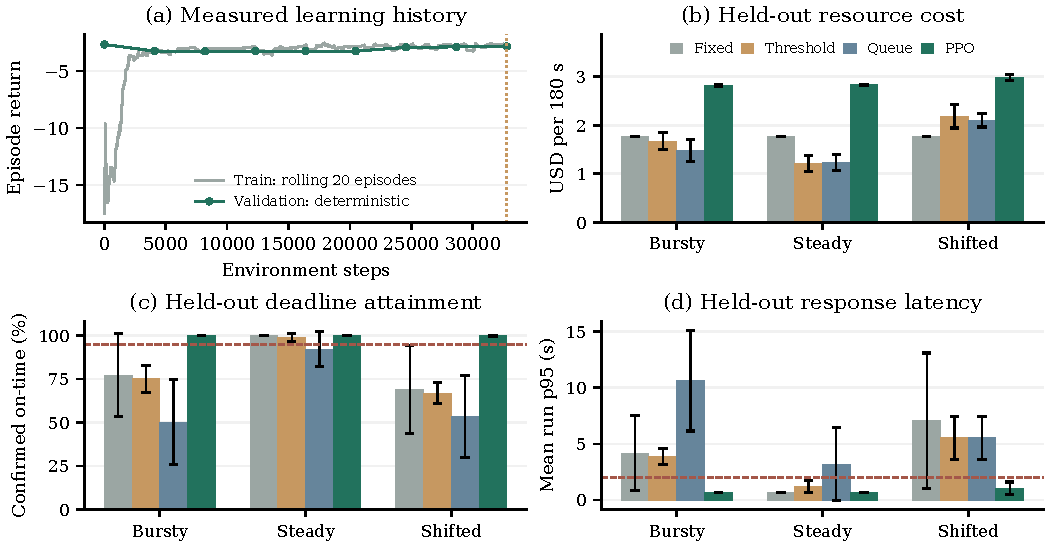
\includegraphics[width=0.94\textwidth]{assignment_results.pdf}
\captionof{figure}{Actual learning history and held-out policy comparison.
Bars show means and 95\% Student $t$ intervals across five request seeds,
conditional on one trained agent. Dashed lines mark the 95\% SLO and 2\,s
deadline. Training and deterministic validation returns are different measures.}
\end{minipage}
\vspace{8pt}
}]

\section{Baselines and Evaluation}
Four-phase nominal rates (requests/s) are
\textbf{bursty}: 2, 12, 3, 20; \textbf{steady}: 8, 8, 8, 8; and
\textbf{shifted}: 15, 2, 22, 4. Each phase rate has a seeded 0.8--1.2 multiplier.
Pricing is \$0.0025 per replica-second and the SLO target is 95\%.

PPO is compared with fixed target four, a utilisation/queue-threshold policy,
and a waiting-token-work policy. The threshold controller is custom, not a
validated Kubernetes HPA implementation. Each policy gets a fresh engine and
the same hashed trace per profile/seed: four policies, three profiles, five
seeds, giving \textbf{60 successful test runs}. Baseline parameters are not tuned.

On-time, late, overdue unfinished, and pending requests are retained.
Confirmed successes give a lower attainment bound; also allowing pending
requests to succeed gives an upper bound. These determine met, violated, or
inconclusive SLO status. Completed-request p95 alone can hide unfinished work.
Completing exactly at the deadline is on time.

\section{Observed Results}
On bursty traffic, PPO averages \BurstyPpoAttainment\% on-time requests versus
\BurstyFixedAttainment\% for fixed, with mean run p95
\BurstyPpoLatency\,s versus \BurstyFixedLatency\,s. That reliability costs
\$\BurstyPpoCost\ versus \$\BurstyFixedCost\ per episode:
PPO spends more rather than demonstrating savings.

On shifted traffic, PPO attains \ShiftedPpoAttainment\% versus
\ShiftedFixedAttainment\% for fixed. Across all profiles, PPO meets the 95\%
SLO in 15/15 runs; fixed, threshold, and queue meet it in 8/15, 5/15, and 3/15.
On steady traffic, threshold already meets the SLO in all five runs at
\$\SteadyThresholdCost\ versus PPO's \$\SteadyPpoCost.
PPO therefore overprovisions easy traffic.

\newpage
Validation return improves from $-3.245$ at early trained checkpoints to
$-2.838$, but remains below the untrained control ($-2.660$).
The evidence supports a cost--reliability tradeoff, not general PPO superiority.
Intervals describe workload variation for one selected agent, not robustness
across training seeds.

\section{Artifacts and Validation}
The repository provides the trained checkpoint, exact traces, training and
validation curves, all test runs, candidate selection, hashes, and settings
under \path{artifacts/rl_study/}. The README documents Python 3.11+ setup,
dependencies, model loading, and reproduction. The module
\path{inferscale.experiments.rl_study} provides \texttt{train},
\texttt{select}, and \texttt{evaluate} commands; full invocations are in the README.

All \textbf{171 Python tests pass}, including hold/cooldown, single-decode timing,
large observation, and checkpoint save/load regressions. Python/FastAPI, SQLite,
and React/TypeScript provide the research application. The RL Study dashboard
shows learning curves, comparisons, and fresh checkpoint replays. Training uses
the CLI; the legacy dashboard training flow remains a placeholder.

{\raggedright
\textbf{Limits.} This is synthetic analytical CPU simulation, not measured GPU
performance or Azure/BurstGPT training. Inference batch control, calibrated
utilisation, multi-seed agent training, and a validated Kubernetes comparison
remain future work.\par}

\end{document}
